\documentclass[12pt,a4paper]{article}

\newcommand{\reporttitle}{Broccoli Drought and Heat Complex Stress Detection and Shelf Life Prediction Based on Spectrometry and Machine Learning}

%%%%%%% 页边距 %%%%%%%%%
\usepackage{geometry}
\geometry{top=2.2cm,bottom=2.2cm}
%%%%%%%% 行距 %%%%%%%%
\linespread{1.5}
%%%%%%%% 字体 %%%%%%%%%
\usepackage[T1]{fontenc} % Output font encoding for international characters
\usepackage[utf8]{inputenc} % Required for inputting international characters
\usepackage{XCharter} % Use the XCharter font
%%%%%%%%%%% 数学公式 %%%%%%%%%%
\usepackage{amsmath}
\usepackage{amssymb}
\usepackage{fourier}
\usepackage{bm}
%%%%%%%%%% Tabular %%%%%%%%
\usepackage{booktabs} 
\usepackage{colortbl} 
\usepackage{xcolor} 
\usepackage{xfrac}
\usepackage{threeparttable} %footnote
%%%%%%%%%% Figure [H]%%%%%%%%%
\usepackage{float}
\usepackage[export]{adjustbox}
\usepackage{enumitem} % Required for manipulating the whitespace between and within lists
\usepackage{graphicx}
\usepackage{gensymb}
\usepackage{lineno}
\usepackage{setspace}
\usepackage{diagbox}
\usepackage{upgreek}
\usepackage{url} 
\usepackage[colorlinks,linkcolor=blue,anchorcolor=blue,citecolor=blue]{hyperref} 
\graphicspath{ {../results/} }

% Harvard-style referencing
\usepackage[comma]{natbib}

\bibliographystyle{agsm}
\setcitestyle{authoryear,open={(},close={)}}

\begin{document}
%%%%%%%%%%%%% front page %%%%%%%%%%%%%%%%
% Last modification: 2016-09-29 (Marc Deisenroth)
\begin{titlepage}

    \newcommand{\HRule}{\rule{\linewidth}{0.3mm}} % Defines a new command for the horizontal lines, change thickness here
    
    %----------------------------------------------------------------------------------------
    %	LOGO SECTION
    %----------------------------------------------------------------------------------------
    
    
\includegraphics[width = 5cm]{./imperial.pdf}\\[0.6cm] 
    
    \begin{center} % Center remainder of the page
    \vspace*{\fill}
    %----------------------------------------------------------------------------------------
    %	HEADING SECTIONS
    %----------------------------------------------------------------------------------------
    % \textsc{\LARGE \reporttype}\\[1.5cm] 
    \textsc{\Large Imperial College London}\\[0.5cm] 
    \textsc{\large Department of Life Sciences}\\[0.5cm] 
    %----------------------------------------------------------------------------------------
    %	TITLE SECTION
    %----------------------------------------------------------------------------------------
    
    \HRule \\[0.4cm]
    { \huge \bfseries \reporttitle}\\ % Title of your document
    \HRule \\[1.5cm]

    %----------------------------------------------------------------------------------------
    %	AUTHOR SECTION
    %----------------------------------------------------------------------------------------
    
    %\begin{minipage}{0.4\hsize}
   

    \reportauthor~(CID: \cid) % Your name

    \vspace{1cm}
    \makeatletter
    Date: \@date \\
    \end{center}


    \vspace*{\fill}% Fill the rest of the page with whitespace

    
    \makeatother
    
    


    \end{titlepage}
    
    
%%%%%%%%%%%%% Declaration %%%%%%%%%%%%%%%%
\begin{center}
\mbox{}\newline\vspace{10mm} \mbox{}\LARGE
{\bf \textit{Declaration}} \normalsize \vspace{2mm}
\end{center}

\noindent
The images of the broccoli head on the conveyor belt used to construct and training the neural network was originally provided by Nathan E. Barlow (Imperial College London), and then the optimized image video was collected by the author and the supervisor, Dr. Oliver Windram (Imperial College London). Besides, Dr. Oliver Windram was mainly responsible for setting up the direction of this project. Acquisition of experimental data, data cleaning, data analysis, method modification, model training, parameter tuning and writing were exclusively performed by the author himself.

\newpage
\linenumbers 
 
%%%%%%%%%%%%%%% Abstract %%%%%%%%%%%%
\mbox{}\newline\vspace{4mm} \mbox{}\LARGE
%
{\bf Abstract} \normalsize \vspace{1mm}
\\
As a non-destructive, and high-efficiency technology, spectroscopy has developed rapidly in crop management for precision agriculture. Many studies on spectroscopic detection of crop stress have made effective progress, including disease detection and water stress, etc. Various vegetation indices have also been established to indicate crops growth status. However, complex growing conditions often cause crops to be affected by multiple stresses, which in turn affect crops yield and quality. Few studies have been conducted on this complex stress, especially the two physiological closely related abiotic stresses, heat and drought. 
\\
\\
Here we took broccoli as our research subject, and collected the hyperspectral reflectance data of its leaves under heat and drought, as well as their combination by spectrophotometer. Then, we explored the spectral characteristics by various vegetation indices, and the results showed that a single vegetation index could hardly be significant in all treatments. Next, we trained four machine learning models, including Logistic regression, Support Vector Machine, Random forest and XGBoost to predict these complex stresses, and the highest AUC can reach 0.9494 by logistic regression. 
\\
\\
Besides, we have developed a visualization method that can dynamically and more intuitively see the significant differences of spectral characteristics between different stress treatments. The strategy is that first, it sets a appropriate wavelength width to reduce the redundancy of hyperspectral information, then randomly searches and accumulates the significant statistical analysis results with the width, and finally outputs the important band peaks dynamically. It can be helpful for spectral image band selection.
\\
\\
And additionally, we also try to combine spectroscopy and deep learning to build a system for predicting the shelf-life of broccoli heads. For now, it can track broccoli heads with ResNeXt to 97.2\% accuracy and segment them with Unet to 99.2\% accuracy, while the signal related to the shelf-life is still in progress.
\\
\\
\textbf{Keywords:} Broccoli; Machine Learning; Spectral feature; Heat stress; Drought stress


%%%%%%%% Word Count %%%%%%%%%%%%%
\begin{flushleft} 
\vspace{3cm}
Word count: 5786.
\newpage
\end{flushleft}


%%%%%%%%%% Contents %%%%%%%%%%%%%%
\newpage
\tableofcontents

%%%%%%%%%% main body %%%%%%%%%%%
\newpage
\section{INTRODUCTION}
The environment in which crops growth is highly dynamic, crops are constantly exposed to various stresses, including abiotic stimuli such as humidity, light intensity and temperature, and biotic stimuli, like pathogens. Correspondingly, to cope with these stresses, plants have evolved a highly dynamic response mechanism, from gene expression regulation to changes in various secondary metabolites, which in turn alter their physiological characteristics, such as enzyme activity, stomatal aperture, photosynthetic rate and transpiration rate \citep{carter1993responses}. Rapid detection of stresses through these physiological changes of crops is particularly important for obtaining high yield and high quality products. Traditional detection methods usually require experts to be able to detect the subtle color changes or a slight droop or curl of plants leaves, which indicate the stress. However, it's generally subjective and time-consuming. In contrast, spectral detection and spectral imaging, as a non-destructive, accurate and efficient method, has developed rapidly both in research and practical application \citep{xue2017significant}. 
\\
\\
The spectral reflectance characteristics and mechanism of leaves have been well summarized \citep{knipling1970physical, gates1965spectral}. When the leaves receive solar radiation, only part of the incident energy is reflected and the rest is transmitted or absorbed for photosynthesis. The typical reflectance spectrum of a leaf is that in the visible region ($0.4-0.7 \upmu$m), the reflectance of leaves is generally very low, especially in red (around $0.63-0.70 \upmu$m) and blue (around $0.45-0.52 \upmu$m), this absorption characteristic is mainly caused by plant pigments. Specifically, the absorption of red primarily contributed from chlorophyll, and the absorption of blue is also involved in carotenes and xanthophylls \citep{gates1965spectral,Rabideau1946THEAA}. Furthermore, the high reflection in near-infrared ($0.7-1.3 \upmu$m) is caused by the internal cellular structure \citep{Mestre1935The,willstatter1907untersuchungen}. Leaf cuticular wax is transparent and hardly reflects solar radiation. Radiation can be transmitted through the epidermis, then dispersed and multiple reflected and refracted in the mesophyll cells and air cavity, where different refracted index between air ($1.0$) and hydrated cell walls ($1.4$) account for these effect \citep{sinclair1968pathway}. 
\\
\\
Previous studies on the application of spectral techniques in plant stress detection have made extensive progress, involving various crops and stress. In biotic stresses, plant disease detection is the most studied. Early in 1982, the diffuse reflectance spectra of potato tubers in the visible and near-infrared bands were measured and analyzed in an attempt to detect the presence of disease before its effects were visible \citep{muir1982experiments}. On top of that, spectral research also progress in the detection of various plant diseases, such as panicle blast, brown planthopper, the bacterial leaf in rice \citep{kobayashi2001detection,prasannakumar2013assessment,yang2010assessment} and yellow rust, powdery mildew in wheat \citep{bravo2003early,cao2013detection}. In abiotic stress, diverse research focus on water stress. Among them, many studies are based on canopy temperature based Crop Water Stress Index (CWSI) measured from infrared thermometry \citep{alchanatis2010evaluation,aladenola2014response,bellvert2016airborne}. The principle of CWSI theory is that transpiration cools the surface of leaves. When soil moisture in the root zone decreases, stomatal conductance and transpiration are weakened, and then leaf temperature increases. What makes this theory popular is its linear relationship between canopy temperature and air temperature and vapor pressure, as well as the development of empirical methods for quantifying crop water stress \citep{idso1981normalizing}. However, though the canopy temperature is very useful for water stress detection, it still has some physiological concerns. In some plants, the diurnal fluctuation in stomatal conductance make the relationship unclear between canopy temperature and stress levels \citep{zarco2012fluorescence}. Moreover, leaf temperature does not directly explain other physiological changes, such as photosynthesis pigments or non-stomatal reduction of photosynthesis under water stress \citep{zarco2013pri}. Therefore, various alternative vegetation indices (VIs) based on the visible and red edge spectral region are developed to capture water stress related signals \citep{berni2009thermal,zarco2013pri,wang2015determining,rossini2013assessing,panigada2014fluorescence,dangwal2016monitoring}. 
\\
\\
Although spectroscopic studies of biotic and abiotic stresses can achieve significant detection under different models, the stress they detect is often single, while in practical production, crops tend to suffer from multiple complex stresses during their growth, such as heat and drought and their combinations, especially in the context of global warming. More importantly, the molecular and physiological mechanisms by which plants respond to heat and drought stress have been extensively studied and they show lots of relevance. Both of them can differentially affect the RNA stability, alter the enzyme activity and disrupt the steady-state of metabolic flux, which in most of cases can cause a common response, oxidative damage \citep{kollist2018rapid,suzuki2012ros, mittler2012plants,mcclung2010ambient}. Moreover, photosynthesis is an important physiological phenomenon affected by drought and heat stress. Drought can lead to stomatal closure and reduces CO$_2$ uptake which makes plants more susceptible to photo damage, also it can induce negative changes in photosynthetic pigments, either increase or decrease chlorophyll content \citep{lawlor2002photosynthetic,anjum2011brassinolide,din2011physiological}. Similarly, exposure to high temperature can also result in a reduction in chlorophyll biosynthesis, thereby disturbing the photosynthetic pigment components \citep{camejo2006changes}. Although many physiological links between plant heat stress and water stress, and it is of great meaningful to detect them in the practical production, little research have been conducted on the relationship between these two stress spectral characteristics and their detection. So it's a great interest and also useful to see how well we can detect the heat stress and drought and their combination from the crops by data mining their spectral characteristics changes.
\\
\\
Alongside this, methodologically, many previous studies on crops stresses detection used statistical discriminant model, especially various VIs. VIs are quite simple and effective algorithms for quantitative and qualitative evaluation of vegetation cover, growth dynamics, and stress levels. But due to different spectral combinations, instrumentation, platforms, and resolutions used, it's hard to have a unified mathematical expression that defines all VIs, customized algorithms needed to developed and tested against specific application requirements \citep{xue2017significant}. In this way, the prediction is often unsatisfactory and the generalization ability somewhat insufficient. Compared with traditional statistical discriminant model, machine learning methods, which developed rapidly in recent years, can generally improve the speed and accuracy of prediction. The main difference between machine learning and statistics lies in their purpose. Statistical models are more designed to infer the relationship between variables, while machine learning models are intended to make the most accurate prediction possible. 
\\
\\
Overall, here we explore the ability to use hyperspectral techniques to detect and differentiate more complex stresses of crops, that is, the combinations of drought and heat, which are highly correlated with each other. Firstly, we calculated some widely known VIs for statistical testing in anticipation of obtaining simple and effective stress-related signals. Then, in order to approach the upper limit of accuracy for detecting different stresses, we apply machine learning strategy, using linear classifiers, such as logistic regression (LG), linear support vector machine (SVM) and tree models, like random forests (RF) and XGBoost for training a robust classifier. On top of this, to increase the interpretability of the model, great efforts had been made in feature engineering. Specifically, we first extract features through dimensionality reduction of Principal Component Analysis (PCA) and Linear Discriminant Analysis (LDA), and explore the importance of features under potential dimensions. Then statistical filter method and model-based embedded method are applied for feature selection. In particular, during these process, in order to better visualize the statistical differences of hyperspectral features under different stress comparisons dynamically, meanwhile be able to adjust the wavelength width to reduce the redundancy of hyperspectral information and provide a reference for specific band selection, a simple visualization search tool has been developed. Finally, the features obtained by these methods are combined to conduct model training, and the prediction effects of drought, heat stress and their combination stress were analyzed by model comparison.
\\
\\
Additionally, in order to optimize the customization of supermarket broccoli products' shelf-life, a computer vision strategy based on deep learning and spectral detection technology is being developed. Now it can track and segment broccoli heads on the conveyor belt through convolution neural network, but futher spectral signals related to shelf-life still need to be analyzed.

\section{MATERIALS AND METHODS}
\subsection{Workflow}
The project mainly includes two parts (Figure \ref{workflow}). The laboratory part is to grow broccolis under control conditions and then perform individual and combined stress treatments, collect spectral images and leaf reflectance spectrum data to explore the signals that can effectively distinguish among them and construct a robust machine learning classifier. The application part is to construct a detection system which can predict the shelf life of broccoli on the conveyor belt through computer vision methods and spectral images under specific bandwidth, which is selected based on the results obtained in the laboratory.
%%%%%%% Figure %%%%%%%%%%#
\begin{figure}[H] 
\centering 
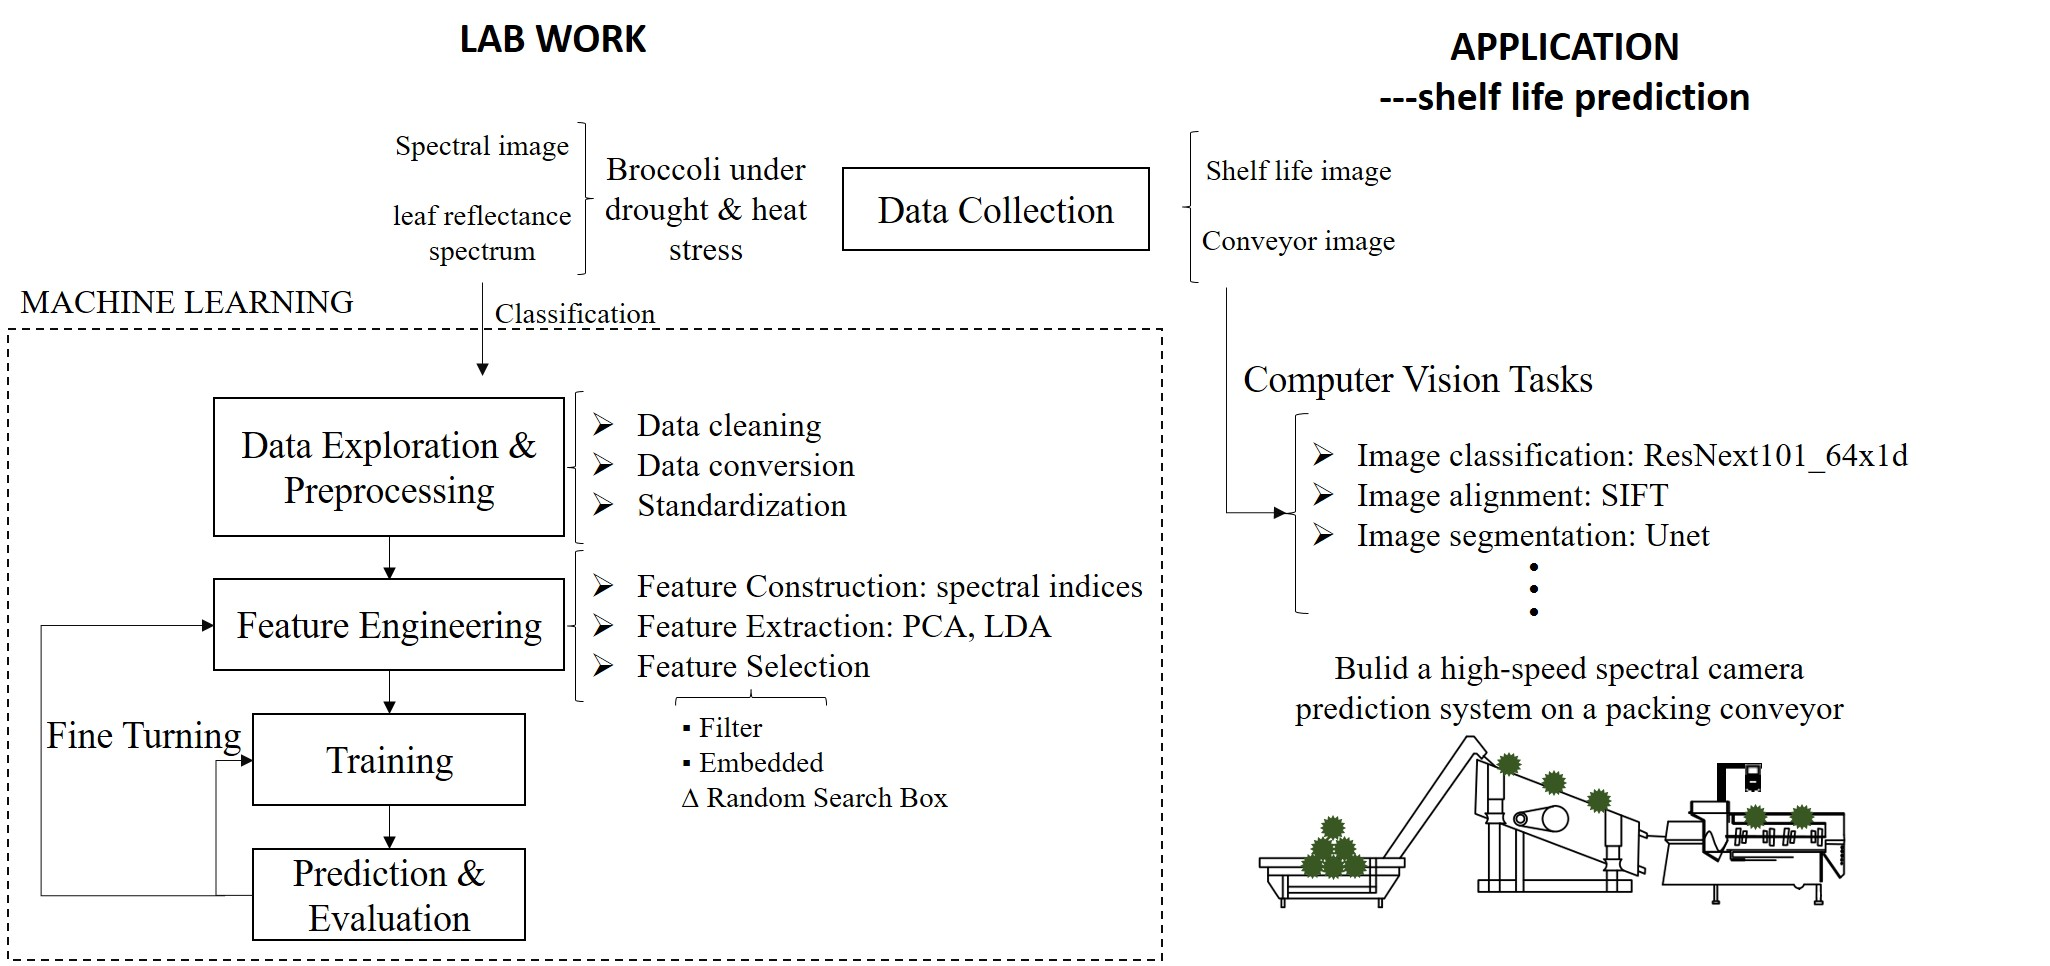
\includegraphics[width=16cm]{./Figure/pipeline.png}
\textbf{\caption{Project workflow}\label{workflow}}
\end{figure}


\subsection{Data Collection}
Broccolis were grown in Control Environment room and greenhouse. The normal growth temperature is controlled at 23 $^{\circ}$C and the humidity is controlled at 60\%, with long daylight (16 hours illumination, 8 hours darkness) treatment, and water is poured every 3 days from the tray to the soil. The whole growth cycle of broccoli takes about three months, during which it needs to be transferred to a suitable pot according to the size of broccoli.
\\
\\
During stress treatment, broccolis were randomly divided into four groups with 8 individuals in each group. They were treated under control, heat stress (27$^{\circ}$C), drought stress (without watering for three days) and the combination of heat and drought stress. Leaf reflectance spectroscopy data was collected by the Ocean Optics FLAME-S-XR1 spectrophotometer in a completely dark room, while the spectral image were collected by Ximea cameras with a specific bandpass filters (FEL0800, FBH650-40) (Table \ref{apparatus}) under the illumination of the corresponding wavelength of the LED lamp. Four days of data were collected until the leaves show a distinct dehydration drooping phenotype. In the open-air greenhouse, spectral images are collected with the same apparatus in a grow tent, in order to eliminate the effect of unstable solar radiation.
%%%%%%%%%%
\begin{table}[H]
    \centering
    \textbf{\caption{Apparatus used in the experiment.}\label{apparatus}}
    \begin{tabular}{cc}
    \toprule​
    \textbf{Item}                        & \textbf{Description}                                               \\ \midrule​
    Camera                               & Ximea 1.3 MP NIR Enhanced Camera MQ013RG-ON\\
    Machine vision lens                  & MVL12M23-12 mm EFL, f/1.4, for 2/3" "                              \\​
                                         & C-Mount Format Cameras, with Lock.                                  \\​ \cline{1-1}
                                         & FEL0800: Ø25.0 mm Premium Longpass Filter,                         \\ ​
                                         & Cut-On Wavelength: 800 nm.                                         \\​
                                         & FBH520: Ø25.0 mm Hard-Coated Bandpass Filters,                     \\​
                                         & Blocking Regions (OD \textgreater 5): 200 - 485 nm, 556 - 1200 nm.  \\​
    Band pass filter                     & FBH650: Ø25.0 mm Hard-Coated Bandpass Filters,                     \\​
                                         & Blocking Regions (OD \textgreater 5),  200 - 611 nm, 690 - 1200 nm. \\​      
                                         & FBH850: Ø25.0 mm Hard-Coated Bandpass Filters,                     \\​ 
                                         & Blocking Regions (OD \textgreater 5),  200 - 805 nm, 896 - 1200 nm. \\​  \cline{1-1}
LED controller                           & Intelligent LED Solutions 12-Channel Light Controller              \\​
LED                                      & 12 Die LED array Full Spectrum 360-955nm                           \\ 
\bottomrule​
    \end{tabular}
\end{table}
\noindent
Broccoli heads for shelf-life prediction come from POLLYBELL FARMS LTD. They are divided into two groups, 18 in each, one of which is stored in cold storage for two weeks, and the other is harvested freshly. They were placed naturally at room temperature and spectral image data were collected every day through the cameras with bandpass filter (FBH520-40, FBH650-40,FBH850-40) and hyperspectral data was collected by spectrophotometer as well until they decay significantly.

\subsection{Vegetation Indices Calculations}
The names, abbreviations, calculation formulas and citations of the various vegetation indices used in this study are as follows, mainly includes commonly used remote sensing indices, chlorophyll-related indices, and indices related to water stress indications.
\begin{table}[H]
    \centering

    \textbf{\caption{Various vegetation indices}\label{vi}}
    \small\addtolength{\tabcolsep}{-5pt}
    \scalebox{0.7}{%
    \begin{threeparttable}[H]

    \begin{tabular}{cccc}
    \toprule
    \textbf{Name}                                                                                         & \textbf{Abbrev.} & \textbf{Equation}                                                                                                                                                                                                               & \textbf{References}\\ \midrule
    \begin{tabular}[c]{@{}c@{}}Ratio \\ vegetation \\ index\end{tabular}                         & RVI     & $R _ { n } / R _ { r }$                                                                                                                                                                                              &  \begin{tabular}[c]{@{}c@{}}\citep{jordan1969derivation}   \\ \citep{pearson1972remote}\end{tabular}        \\ \\
    \begin{tabular}[c]{@{}c@{}}Normalized\\ difference\\ vegetation\\ index\end{tabular}         & NDVI    & $\left( R _ { 800 } - R _ { 680 } \right) / \left( R _ { 800 } + R _ {680} \right)$                                                                                                                                        &  \begin{tabular}[c]{@{}c@{}}\citep{rouse1974monitoring}   \\ \citep{tucker1979red}\end{tabular}         \\ \\
    \begin{tabular}[c]{@{}c@{}}Enhanced\\ vegetation\\ index\end{tabular}                        & EVI     & $2.5 \left( R _ { n } - R _ { r } \right) \left( R _ { n } + 6 \cdot R _ { r } - 7.5 \cdot R _ { b } + 1 \right)$                                                                                                  &       \citep{huete2002overview}       \\ \\

    \begin{tabular}[c]{@{}c@{}}Chlorophyll\\ vegetation\\ index\end{tabular}                     & CVI     & $R _ { n } \cdot R _ { r } / R _ { g } ^ { 2 }$                                                                                                                                                                      &       \citep{vincini2008broad}       \\ \\
    \begin{tabular}[c]{@{}c@{}}Chlorophyll\\ index - green\end{tabular}                          & CI-G    & $R _ { n } / R _ { g } - 1$                                                                                                                                                                                          &           \citep{gitelson2003relationships}   \\ \\
    \begin{tabular}[c]{@{}c@{}}Chlorophyll\\  index - red edge\end{tabular} & CI-RE   & $R _ { n } / R _ { re } - 1$              &      \citep{gitelson2003relationships}        \\ \\
        
    \begin{tabular}[c]{@{}c@{}}Photochemical\\reflectance\\index\end{tabular}                      & PRI    & $\left( R _ { 531 } - R _ { 570 } \right) / \left( R _ { 531 } + R _ { 570 } \right)$ &      \citep{gamon1992narrow}        \\ \\
    \begin{tabular}[c]{@{}c@{}}Water index \end{tabular}          & WI  & $R _ { 900 } / R _ { 970 }$                                &       \citep{zarco2003water}       \\ \\

    \begin{tabular}[c]{@{}c@{}}Structure\\independent\\pigment index\end{tabular}                                   & SIPI    & $\left( R _ {800 } - R _ { 445 } \right) / \left( R _ { 800 } + R _ { 680 } \right)$       &        \citep{penuelas1999reflectance}     \\
                                                                                       \bottomrule    
    \end{tabular}

    \begin{tablenotes}
    $R _{\lambda}$ is the reflectance at wavelength $\lambda$; $n, re, b, g$ and $r$ represent NIR ($760-900$ nm), RE ($700-730$ nm), blue ($450-520$ nm), green ($520-600$ nm) and red ($630-690$ nm) respectively.
      \end{tablenotes}
     \end{threeparttable}
    
   }

\end{table}

\subsection{Machine Learning}
Machine learning generally includes several steps in practical operation, such as data collection and preprocessing, model selection, training, evaluation and repeatedly fine-tuning until a good prediction effect is achieved (Figure \ref{workflow}). In the data preprocessing stage, Z-score standardization is applied to simplify the calculation and the categorical data is one-hot encoded. In the strategy of training algorithms, firstly, LG, SVM, RF and XGBoost algorithm were trained to fit the raw data and obtained the baseline score, and then the performance of the models were optimized by feature engineering and parameters adjustment. Most of the code used in this process is based on the API provided by scikit-learn \citep{scikit-learn}.

\subsubsection{Model Fitting}
Logistic regression: the binomial logistic regression model is a classification model, which is represented by the conditional probability distribution $ P(Y|X) $, in the form of parameterized logistic distribution. Here, the value of $X$ is a real number, and the random variable $Y$ takes a value of 0 or 1, then we estimate the model parameters by supervised learning. The binomial logistic regression model is the conditional probability distribution as follows: 
\begin{displaymath}
    P(Y=1|x) = \frac{\exp(w\cdot x)}{1+\exp(w\cdot x)}
\end{displaymath}
\begin{displaymath}
    P(Y=0|x) = \frac{1}{1+\exp(w\cdot x)}
\end{displaymath}
Here, $x$ is the input vector, $w$ is the weight vector and $Y$ is the output vector, $Y\in{\{0,1\}}$, $ x = (x^{(1)},x^{(2)},...,x^{(n)},1)^{T} $, $ w = (w^{(1)},w^{(2)},...,w^{(n)},b)^{T} $. By comparing the probability of $P(Y=1|x)$ and $P(Y=0|x)$ can finally determine the category. The cost function of logistic regression can be derived by the method of maximum likelihood estimation, which is known as the average of cross-entropy loss. Meanwhile, in order to prevent over-fitting, the L1 or L2 regularization terms was added during the optimization process.
\\
\\
SVM: the main idea of SVM is to find the decision boundary with the largest classification interval between two different categories, which means that a hyperplane separating classes in the feature space is defined by the principle of maximum margin between the closest different data points, also known as support vectors. For simple linear separability problems, it can be described as an optimization problem by mathematical formulas as follows:  
\begin{displaymath}
    \max _ { w,b } \left[ \min _ { x _ { i } } \frac { y _ { i } \left( w\cdot x _ { i } + b \right) } { \| w \| } \right]
\end{displaymath}
The minimized item represents the distance from the support vectors to the decision boundary with sign, known as geometry margin. After derivation and transformation, and allow the SVM to ignore some noise, that is, allow some data points' functional margin less than $1$, a slack variable ($\xi _ { i } \geq 0$) is introduced to allow some wrong classification. correspondingly, a penalty term is needed to add to the objective function to limit the slack variable, and here is the basic linear separable SVM:
\begin{displaymath}
\begin{array} 
    { c } { \min \frac { 1 } { 2 } | | w | | ^ { 2 } + C \sum _ { i = 1 } ^ { m } \xi _ { i } } \\ { \text { s.t. } y _ { i } \left( w ^ { T } x _ { i } + b \right) \geq 1 - \xi _ { i }  ( i = 1,2 , \ldots m ) } \\ { \qquad \xi _ { i } \geq 0 \quad ( i = 1,2 , \ldots m ) } 
\end{array}
\end{displaymath}
Finally, the problem can be resolved by Lagrange Duality and SMO algorithm \citep{Platt98sequentialminimal}. In addition, kernel mapping has also been tried to verify the model's performance under nonlinearly separable conditions.
\\
\\
Ensemble methods: Random Forests and XGBoost \citep{chen2016xgboost}, both are based on decision tree model, they use the strategy of bagging and boosting respectively, which can help to prevent high variance and high bias. Random forest mainly consists of two stochastic processes, random sampling of samples and features to construct many decision trees that are independent of each other. The final prediction results are summarized by voting strategy. As for XGBoost, it's an algorithm developed from gradient boosted decision trees and designed for speed and performance. It's widely used in many competitions and achieved good grades.
\\
\\
Metric: ROC curve (receiver operating characteristic curve) is a graph showing the performance of a classification model at all classification thresholds. The curve plots the points of (True positive Rate, False Positive Rate) at different classification thresholds. Lowering the classification threshold classifies more items as positive, thus increasing both False Positives and True Positives. Area under the ROC Curve (AUC) measures the entire two-dimensional area underneath the entire ROC curve. AUC is desirable for its scale-invariant and classification-threshold-invariant.
\\
\\
When multi-classification is performed on logistic regression and SVM, "one to the rest" strategy is applied. All the models are validated by 6-fold cross-validation, and ROC and AUC is used as the metric for model evaluation.

\subsubsection{Feature Engineering}
Generally, data and features determine the upper bound of machine learning, whereas models and algorithms only approximate this upper bound. The purpose of feature engineering is to extract effective features and remove redundant features, also it can make features machine readable and contextually relevant. It basically includes feature extraction, feature construction and feature selection (Figure \ref{workflow}). Separately, feature extraction mainly uses dimension reduction methods such as PCA and LDA. Feature construction is to construct new features based on previous expertise. Feature selection methods can be roughly divided into three types:

\begin{itemize}[noitemsep] % [noitemsep] removes whitespace between the items for a compact look
    \item Filter: scoring each feature according to divergence, correlation, etc., and then set a threshold for selection feature. 
    \item Embedded: use some machine learning algorithms and models to train and get the coefficients of each feature, select features according to the coefficient, kind of similar to the filter method, but models are trained to determine the pros and cons of features. Specifically, multi-method ensemble selection \citep{feilhauer2015multi} was modified from the regression problem and later adapted to the classification problem.
    \item Wrapper: recursive elimination feature method, due to the high computational complexity and the long execution time of the algorithm, it is not adopted here.
\end{itemize}
In addition, in order to find a suitable bandpass filter for the camera, a search box with specific bandwidth was used to repeatedly and randomly select features, and the importance of features is sorted by simple ANOVA and TukeyHSD significance test. Finally, the graph is plotted by accumulating significant $(p<0.05)$ bandwidth features.

\subsection{Computer Vision}
The project involves computer vision tasks such as image classification, segmentation, and image alignment. Specifically, image alignment was performed by classic Scale-invariant feature transform (SIFT) \citep{lowe1999object}, Image classification and segmentation are mainly accomplished by the transfer learning of convolution neural network (Figure \ref{Conv}).

\begin{figure}[H] 
    \centering 
    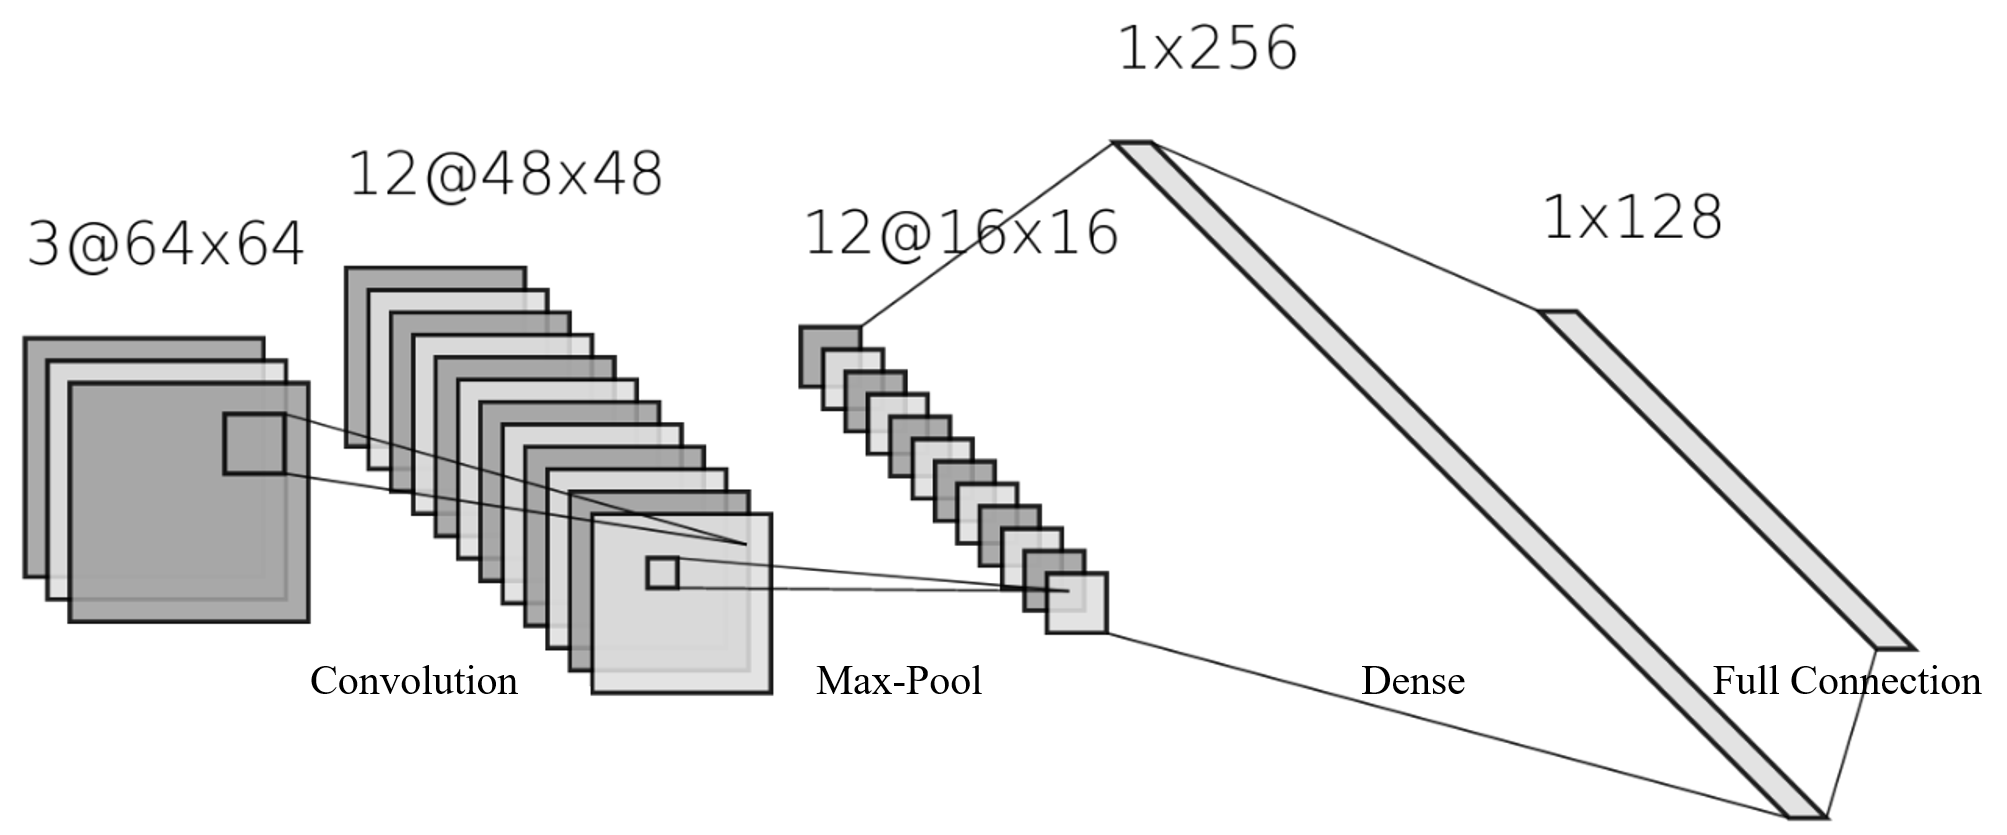
\includegraphics[width=14cm]{./Figure/Convnet.png}
    \textbf{\caption{Structure of a simple convolution neural network}\label{Conv}}{An image was taken as input (for example, a RGB image, normally three channels), then through the calculation with the multiple kernels' parameters and activation functions (usually ReLu) in convolution layer, and the downsampling process in pooling layer, can achieve the purpose of weight sharing and parameter reduction. Finally, the results are expanded and classified by the fully connected layer and the softmax function. In the figure, the number in front of @ is the number of channels, and the number followed by is the height and width of pixels.}
\end{figure}
\noindent
More specifically, Image classification was implemented by ResNeXt \citep{Xie2016}, developed by UC San Diego and Facebook AI Research, while Image segmentation was implemented by Unet \citep{ronneberger2015u}. The training was conducted on GPU P1000, the optimizer for the neural network is Adam \citep{kingma2014adam}, the cost function is cross-entropy, and cyclical learning rates \citep{smith2017cyclical} was used, Most of the code is based on the API provided by Pytorch, fastai library \citep{howard2018fastai}, and opencv.

\section{RESULTS}
\subsection{Data}
To study the spectral characteristics of drought stress, heat stress, and their combination, Leaf reflectance non-image hyperspectral data (Figure \ref{Raw}a) and spectral images of two channels (Figure \ref{Raw}b) were collected. We select the data of the day when the broccoli just appeared phenotype under the stress to ensure the treatment effect and maximize model performance. Under the control and heat conditions, the broccolis have no obvious phenotype, while under drought and combined stress treatment, the broccoli leaves are a little drooping due to dehydration, and the combined stress is slightly more obvious than the drought (Figure \ref{Raw}b).
\begin{figure}[H] 
    \centering 
    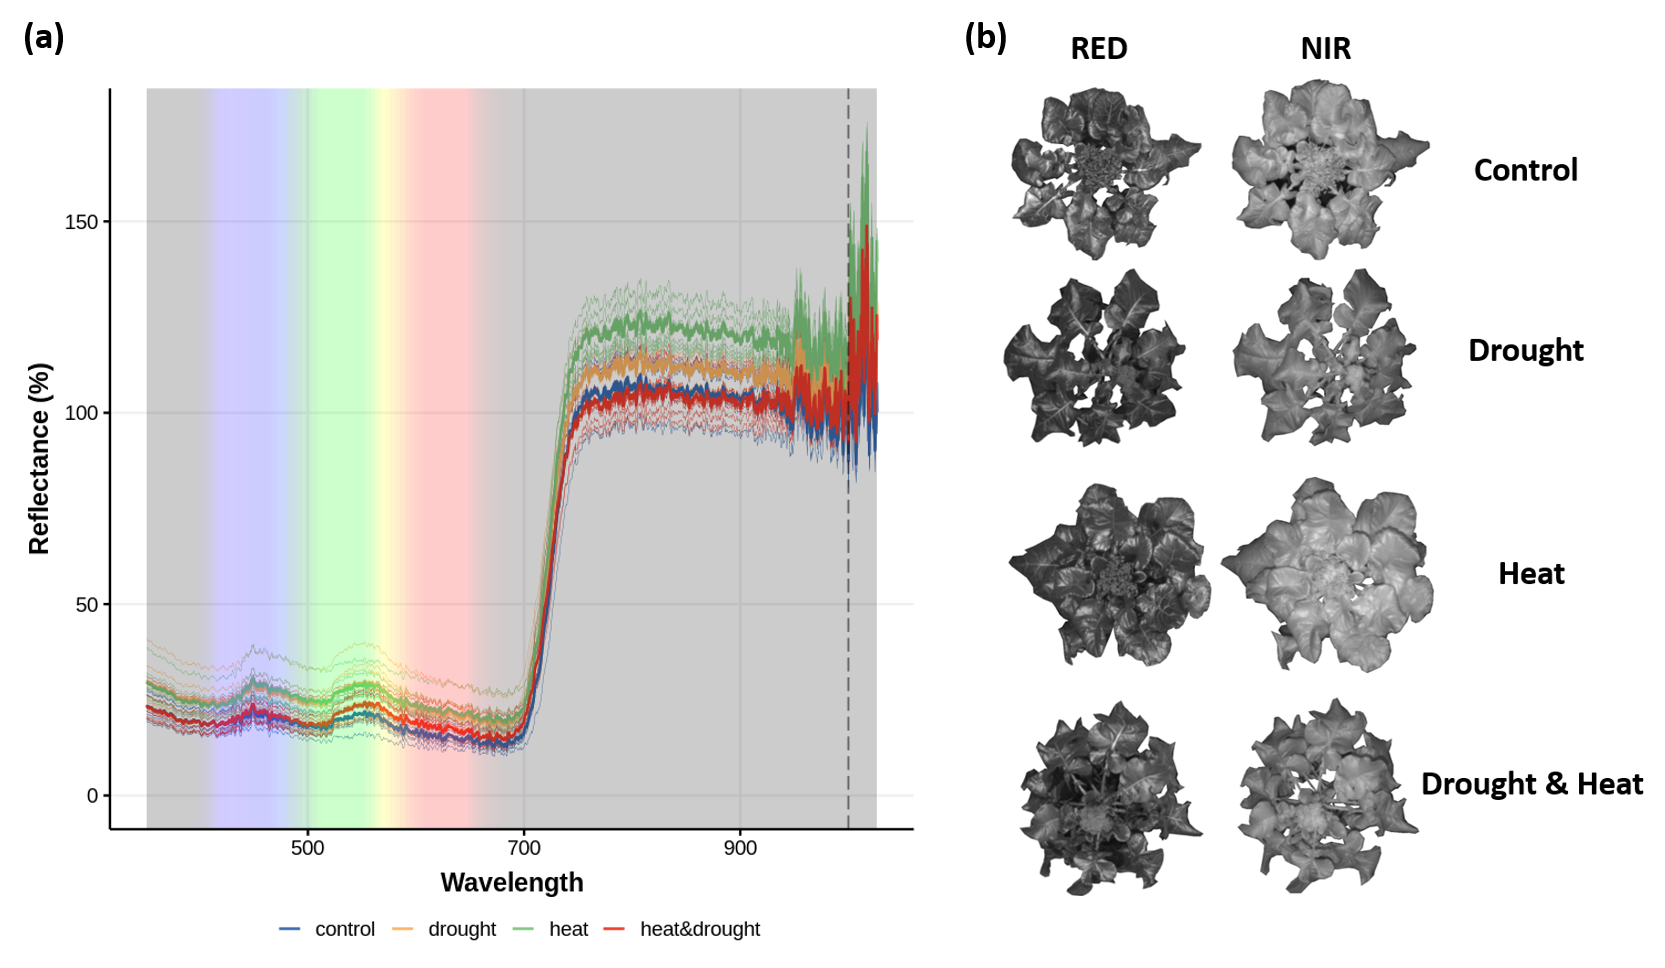
\includegraphics[width=16cm]{./Figure/0401RAWplot.png}
    \textbf{\caption{hyperspectral non-imaging data and spectral iamge data of broccoli under heat and drought stress broccoli under heat and drought stress}\label{Raw}}{(a) is the hyperspectral data of broccoli leaves detected by spectrophotometer in dark environment, the vertical axis represent their relative reflectivity. The thin line is the average of 80 hyperspectral scans per sample, and the thick line is the average of all samples in different treatments. The right side of the dashed line was discarded is subsequent processing due to abnormal signal fluctuation. (b) is the spectral images taken by the camera with red bandpass filter (CWL = 650 nm, FWHM = 40 nm) and near infrared bandpass filter (> 800 nm), under the illumination of the corresponding band of LED.}
\end{figure}
\noindent
For the hyperspectral data of the leaves (Figure \ref{Raw}a), we scanned the leaves of 28 samples (7 samples per treatment), collected data every 10 scans, and finally got 80 data points per sample. The plots between treatments overlap to each other, so there is no clustering to get a simple discriminant pattern. However, the overall trend of the broccoli leaves reflectance spectrum can still be clearly seen. Small peaks at the blue and green-yellow junctions in the visible region, and well-known small valley in the red and strong reflection rate shifting in the near-infrared. These are mainly caused by the pigment and cell structure of broccoli \citep{gates1965spectral}. It's also worth pointing out that the average reflectance of the heat treatment appears to be generally higher than other treatments in the near-infrared.

\subsection{Vegetation Indices}
For the sake of looking for a simple and effective algorithm to distinguish four different treatments, several common spectral indices were calculated under different stress (Figure \ref{vif}). Specifically, basic vegetation index RVI, is based on the phenomenon that leaves absorb relatively more red than infrared light. It's widely used for green biomass estimations \citep{jordan1969derivation}. NDVI is the most widely used VI to characterize canopy growth and vigor \citep{karnieli2010use}. EVI was introduced to correct soil and atmospheric effects on NDVI \citep{xue2017significant}. As for CVI, CI-G and CI-RE, they are to some extent related to chlorophyll content \citep{gitelson2003relationships, vincini2008broad}. and for PRI, WI and SIFI have been proven to be effective of water status in some species \citep{ihuoma2017recent, katsoulas2016crop}.
\\
\\
The results show that significant differences between every two treatments can't be simply obtained from a single index. The results with significant differences also show different forms of band feature calculation methods, which is difficult to establish a unified pattern, suggesting that more complex models are needed.
\begin{figure}[H] 
    \centering 
    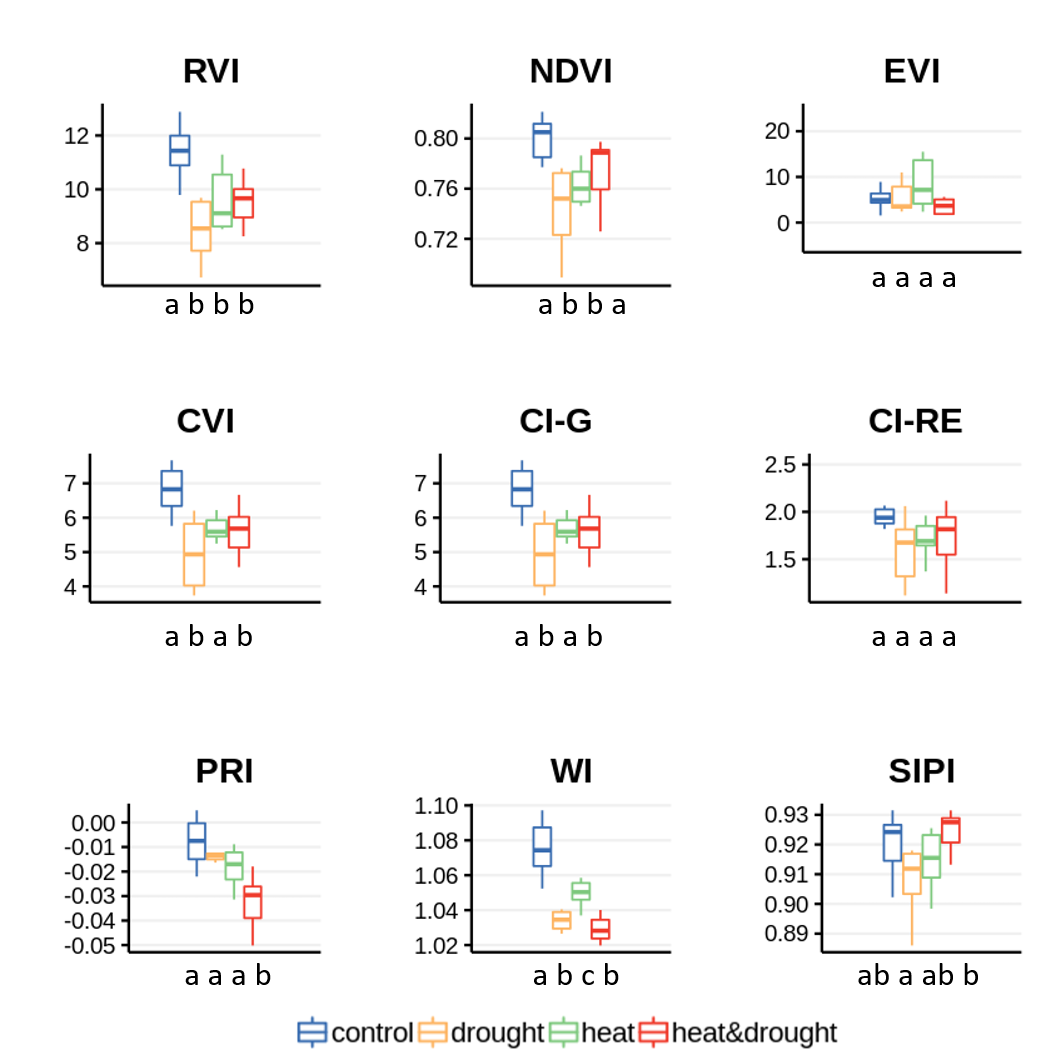
\includegraphics[width=13cm]{./Figure/vi.png}
    \textbf{\caption{Various vegetation indices under different stresses}\label{vif}}{Seven samples per treatment, the equation for calculating vegetation index refers to Tabel \ref{vi}. Normality test was implemented by shapiro test, and homogeneity of variance test was implemented by Barlett test before using ANOVA and Tukey's HSD for post-hoc analysis. Different letters under the x-axis represent sigificant differences ($p < 0.05$).}
\end{figure}

\subsection{Dimensionality Reduction}
There may be multi-collinearity between hyperspectral features, that is variables may be correlated. Meanwhile, too many variables may hinder the pattern for model fitting, and it may also involve a lot of redundant information. Therefore, dimensionality reduction was used to reduce variables, speed up computation and extract effective information hidden in the data.
\begin{figure}[H] 
    \centering 
    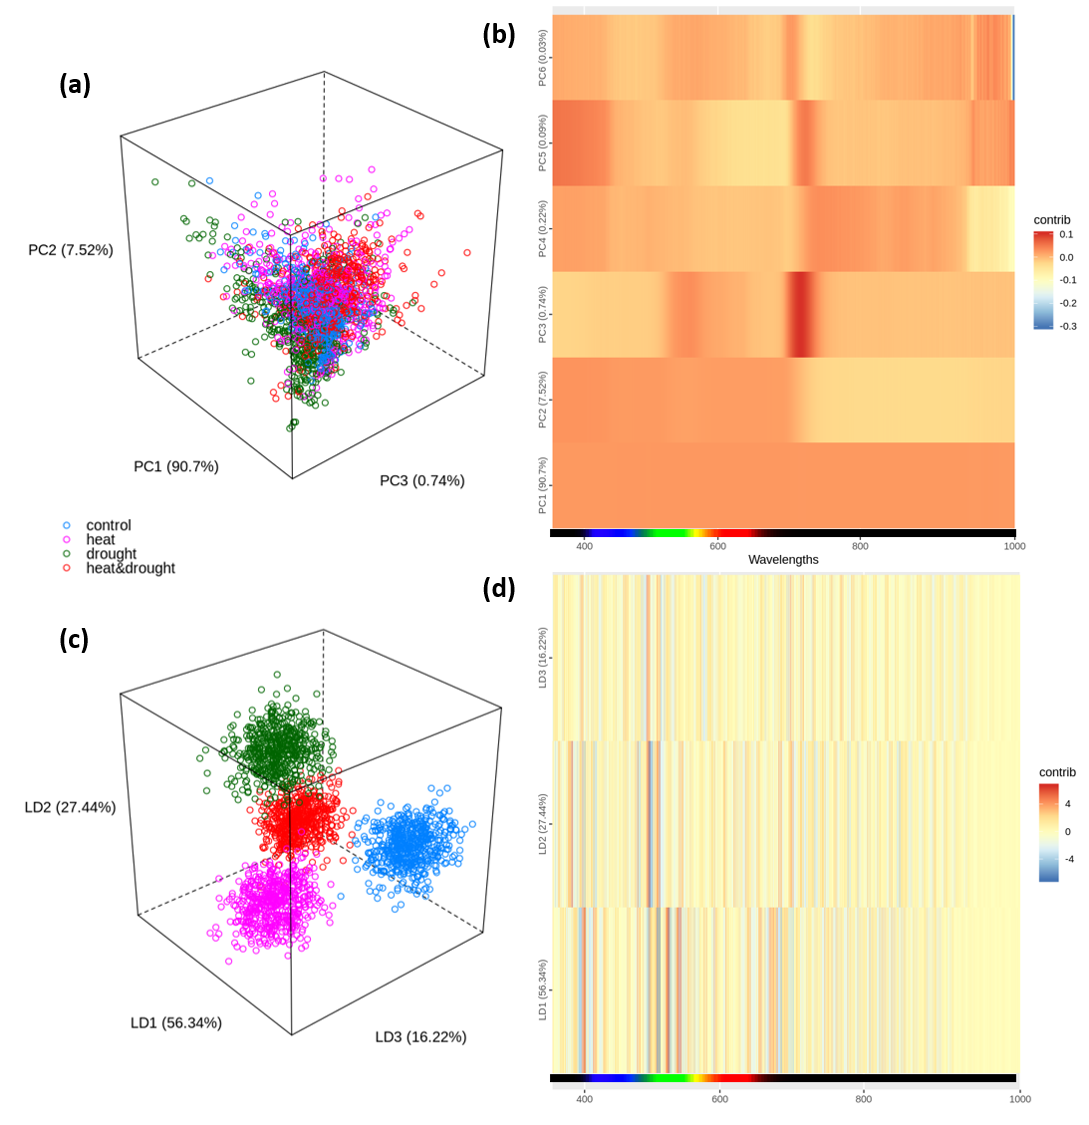
\includegraphics[width=13cm]{./Figure/dim.png}
    \textbf{\caption{Feature dimensionality reduction by PCA and LDA}\label{dim}}{(a) and (b) are the distribution of the samples in the first three principal component dimensions, in which the values in the coordinate axis are the explanatory rates of the overall differences; Heat maps (c) and (d) indicate the correlation between each wavelength and each component.}
\end{figure}
\noindent
The results of unsupervised dimensionality reduction PCA show that, when the variables are mapped to the linear-independent direction of maximum variance, clustering between different treatment is not effective (Figure \ref{dim}a). Surprisingly, PC1 explains $90.7\%$ of the variance, and the contribution of each wavelength seems to contribute equally to it, possibly due to the systematic errors. In PC2, the visible light region contributes a larger variance, and there are two specific narrow bands in PC3 that are positively correlated with it (Figure \ref{dim}b). On the other hand, LDA, the supervised dimension reduction method, can completely separate the different treatments (Figure \ref{dim}c). In these components, the green (around $520 nm$) and red edge (around $680 nm$) wavelength may be important to separate each stress treatment in the principal components (Figure \ref{dim}d).

\subsection{Feature Selection}
In order to remove irrelevant features, reduce over-fitting in the process of model training, and find explanatory wavelengths that can effectively distinguish different treatments. We explored several feature selection methods as followed.
\begin{figure}[H] 
    \centering 
    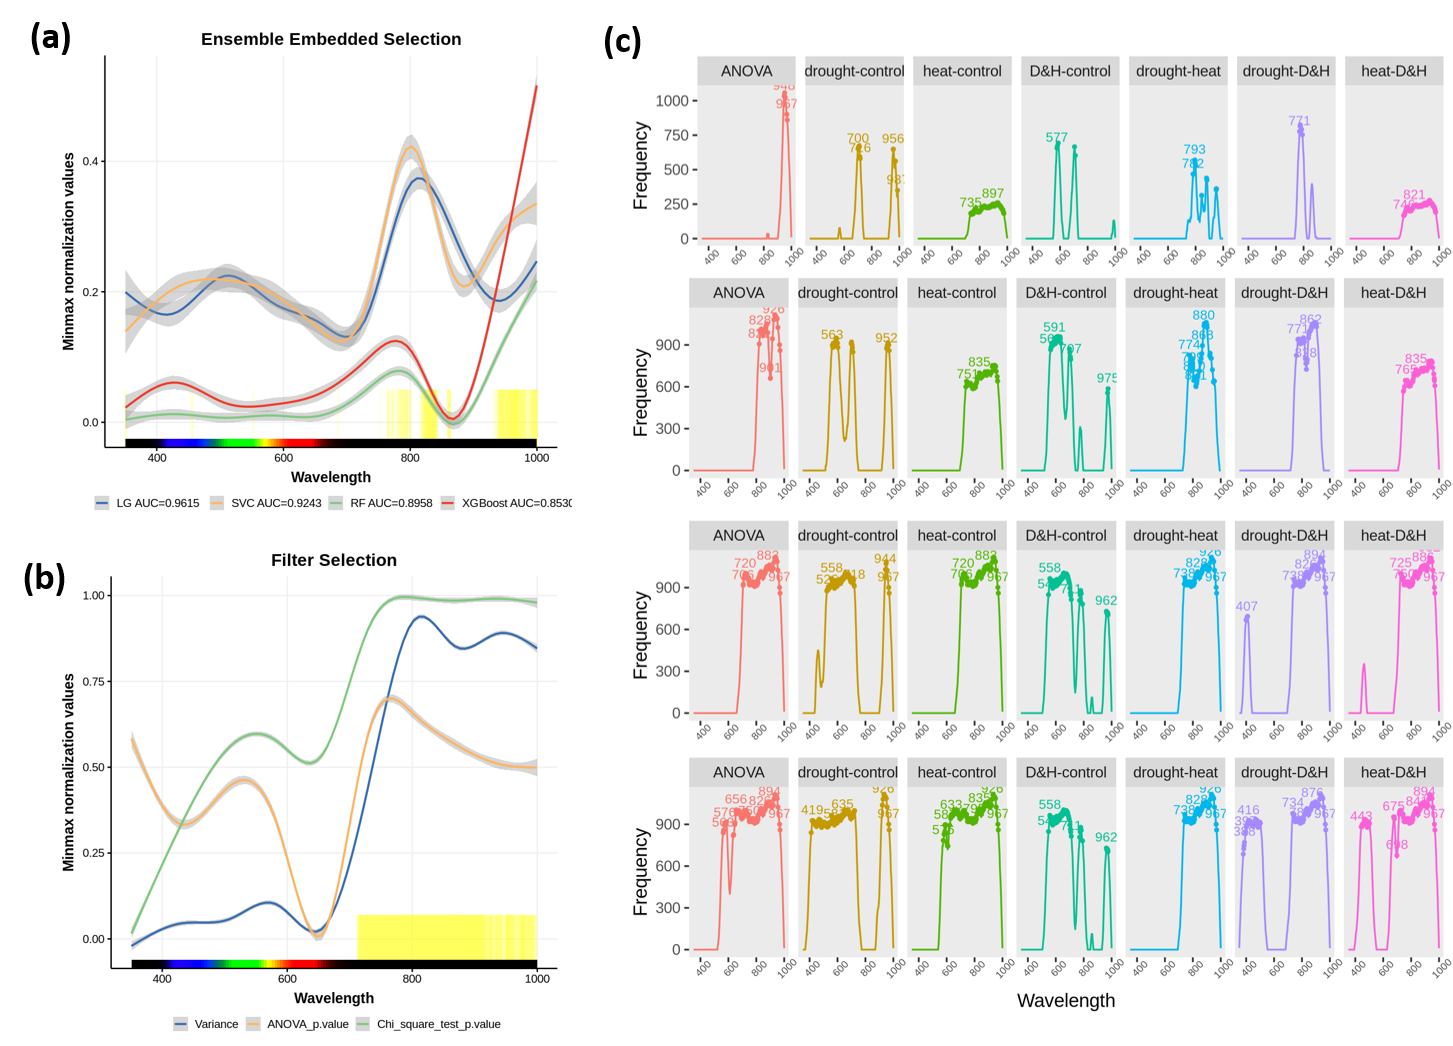
\includegraphics[width=13cm]{./Figure/SL.png}
    \textbf{\caption{Feature Selection}\label{SL}}{For visualization purposes, all coefficients are min-max normalized. In (a) and (b), the gray shadows show the confidence intervals, and the yellow vertical lines indicate the important features upon the setting threshold (Filter: the coincidence of the top 50\% importance features of each filter. Embedded: AUC weighted average of coefficients of each model). (c) From top to bottom shows the significant difference of wavelengths between different treatments dynamically, the earlier the peak appears, the more significant it is, the number on the graph represents where the peak is.}
\end{figure}
\noindent
Filter and Embedded methods are commonly used feature selection methods in machine learning. The results of the Filter method (Figure \ref{SL}b) show that the variance, chi-square test and the ANOVA of each wavelength are coincident upon threshold in the near-infrared region. As for the modified ensemble method \citep{feilhauer2015multi}, the correlation coefficient or feature importance obtained by fitting the LG, SVM, RF and XGBoost are weighted with their AUC scores, then set their average plus standard deviation as threshold. And the features upon the threshold are maily include two near-infrared fragments and other narrow fragments in visible light (Figure \ref{SL}a).
\\
\\
However, although we have acquired some features through these two methods, it's still not convincing enough for us to explain the relationship between features and the treatments. For the embedded method, the generalization ability could be constrainted by the algorithm itself. As for Filter method, it mainly focuses on the correlation between individual features and treatments. The advantage of this method is that it is efficient in computing and robust to over-fitting problems, but it tend to choose redundant features because they do not consider the correlation between features. Moreover, for both methods, the detail of features importance in the pairwise relationship of different treatments remain unclear. And more significant, if these hyperspectral signals are applied to practice, continuous bandwidth signals make more sense for spectral cameras.
\\
\\
So here, we developed a tool to better visualize and select significant continuous wavelengths. It works like this. First, we set a bandwidth (here, 40 nm), then randomly and iteratively search for the wavelength of this bandwidth in the hyperspectral signals, and take the average of the signal for variance analysis. Record the significant band ($p < 0.05$), and finally count the number of times the significant band appears and dynamically display based on the magnitude of the significance (Figure \ref{SL}c). Here, based on the results, we roughly selected 409-429 nm, 558-577 nm, 700-896 nm and 926-967 nm wavelengths for latter model training.

\subsection{Models}
Four kinds of machine learning model were applied to fit the different treatments' hyperspectral data, each treatment has $7$ samples, 80 scans per sample and each scan is the average of 10 scans. A total of $4\times7\times80$ data was used for model fitting, with 6-fold cross-validation and ROC-AUC as an evaluation metric.
\\ \\
Results (Table \ref{auc}) shows that in the fitting of the original data, the linear classifier LG and linear SVM fit well, while tree-based model performance is relatively poor, mainly because the number of features is too large. Too much redundant information makes the tree model easier to overfit. After removing some noise from PCA, the performance of the tree models are improved, but the effect of LDA is less pronounced. Furthermore, through the result of feature selection in the previous step, the models were trained with 409-429 nm, 558-577 nm, 700-896 nm and 926-967 nm wavebands, and the performance of the tree model is further improved.
\begin{table}[H]
    \textbf{\caption{AUC of 4 machine learning models under different features}
    \label{auc}}
    \centering
    \begin{threeparttable}[H]
    \begin{tabular}{@{}ccccc@{}}
    \toprule
                  & \textbf{LG} & \textbf{SVM} & \textbf{RF} & \textbf{XGBoost} \\ \midrule
    raw           & 0.9494         & 0.9122       & 0.7794      & 0.8235           \\
    LDA           & 0.6826         & 0.6817       & 0.6710      & 0.6655           \\
    PCA           & 0.8509         & 0.8507       & 0.8285      & 0.9005           \\
    Selection     & 0.9108         & 0.8758       & 0.7438      & 0.8026           \\
    Selection+PCA & 0.9155         & 0.8754       & 0.8767      & 0.9096           \\ \bottomrule
    \end{tabular}
    \begin{tablenotes}
        \footnotesize{Selection stands for 409-429 nm, 558-577 nm, 700-896 nm and 926-967 nm wavelengths.}
          \end{tablenotes}
    \end{threeparttable}
\end{table}

\begin{figure}[H] 
    \centering 
    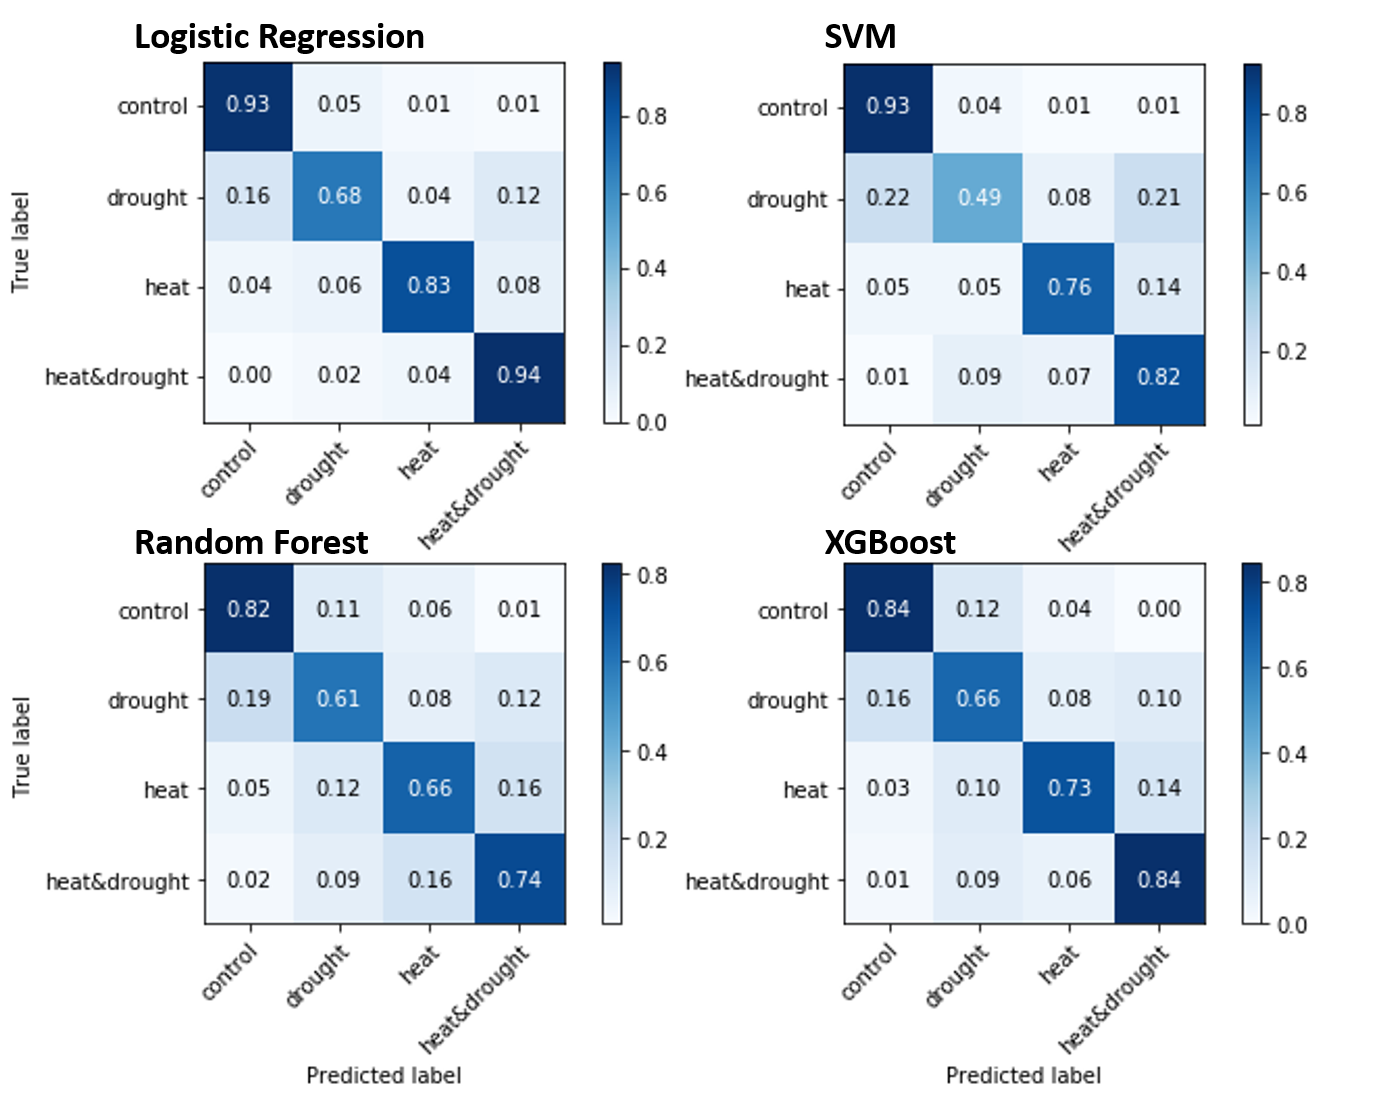
\includegraphics[width=13cm]{./Figure/CM.png}
    \textbf{\caption{The confusion matrix}\label{CM}}{The prediction effect when the four models have the best AUC. Ture label refers to the original category of the data, and the predicted label is the category predicted by the model. The number in the box represents the accuracy, calculated by the number of predicted samples divided by the total number of samples for each category}
\end{figure}
\noindent
Next, we observe their confusion matrix (Figure \ref{CM}) when they have their best AUC. The prediction performance of the four models is similar for different treatments. Among them, the control and combined stress treatments have the best predictive effect, followed by the heat stress, while surprisingly, the drought stress, it has visually obvious symptom (droopy leaves), is the worst, and its mispredictions tend to appear more in control and combined stress.

\subsection{Shelf Life Prediction}
\begin{figure}[H] 
    \centering 
    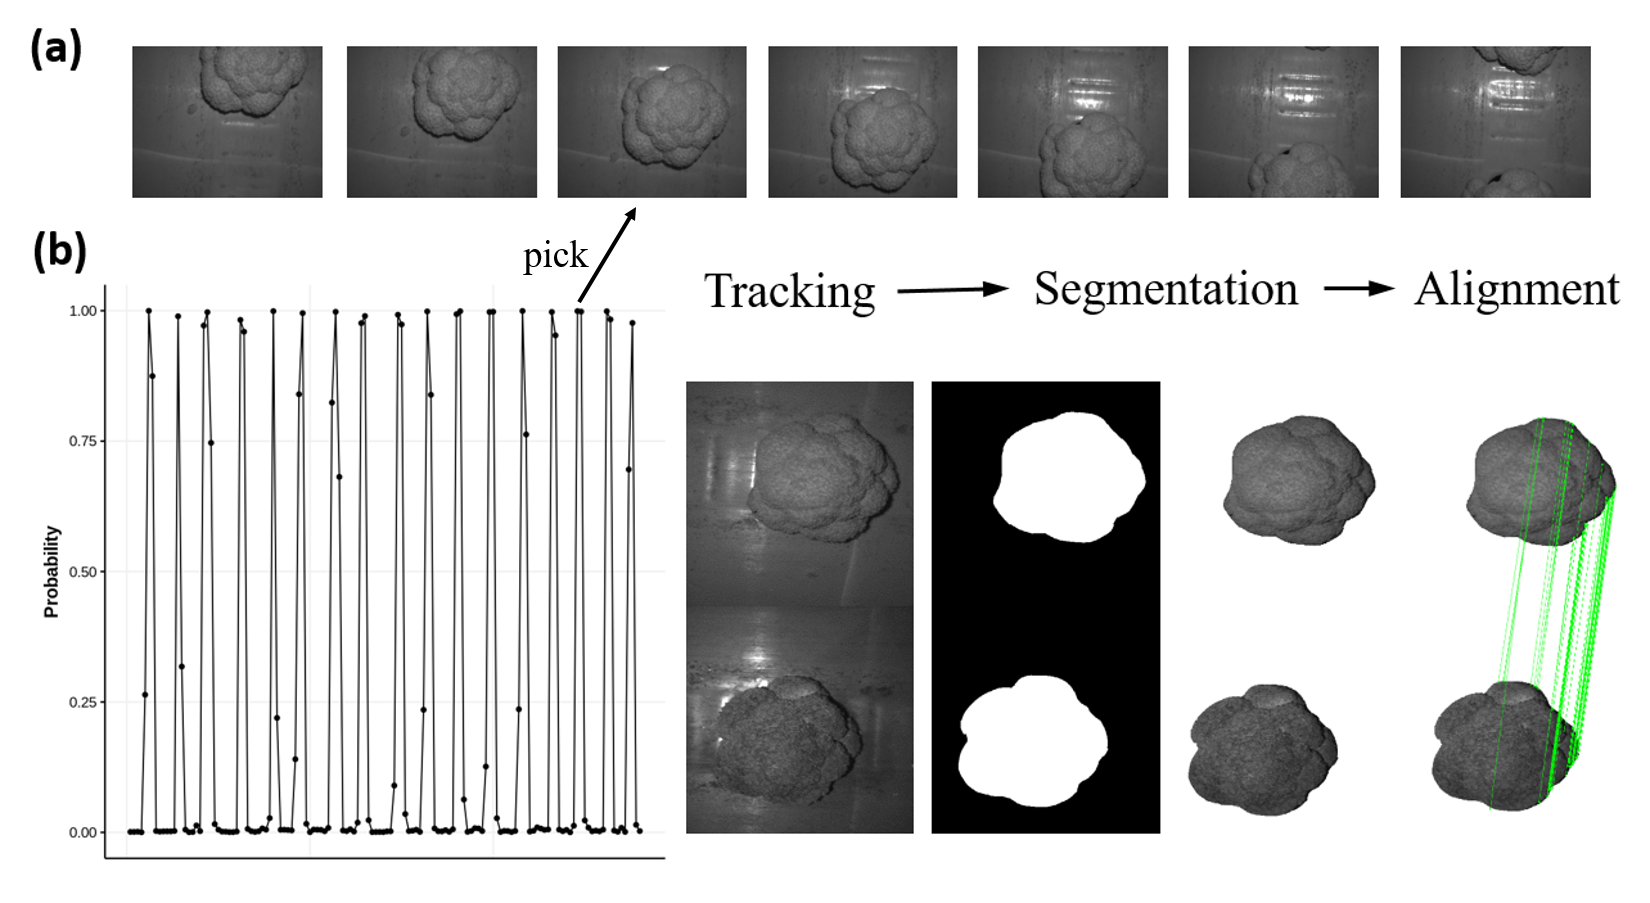
\includegraphics[width=13cm]{./Figure/DL.png}
    \textbf{\caption{Processing of broccoli head images on conveyor belt}\label{deeplearning}}{(a) from left to right is a broccoli time series images on a conveyor belt in the near-infrared channel; (b) is the ResNeXt prediction to track whether broccoli is in the middle of the lens, the closer the prediction probability is to 1, the more likely the broccoli head is in the middle of the lens. Select the image with the largest predicted probability between the two valleys, then segment by Unet and matched by SIFT.}
\end{figure}
\noindent
To predict the shelf life on the broccoli packaging conveyor, we collected thousands of broccoli spectral images (Figure \ref{deeplearning}a) with high-speed band-specific filter cameras and specific waveband LED lights, and then we labeled $5708$ broccoli images to tell whether the broccoli head was in the middle of the lens, so that we can capture the spectral signal of the whole head. And through data augmentation, with limited computing resources, a simple classifier can be constructed by transfer learning of ResNext101\_64 \citep{Xie2016} convolution neural network, which can easily achieve an accuracy of $97.2\%$. By setting a lower threshold of predicting probability, then we can select the highest probability of broccoli head images between the two valleys to track broccolis (Figure \ref{deeplearning}b). After that, for the sake of removing the influence of the background, we labeled $492$ masks for broccoli images segmentation, the Unet \citep{ronneberger2015u} was trained to reach $99.2\%$ accuracy. Next, through the powerful SIFT operator \citep{lowe1999object}, the images of different channels can be aligned for subsequent shelf-life related signals analysis.
\begin{figure}[H] 
    \centering 
    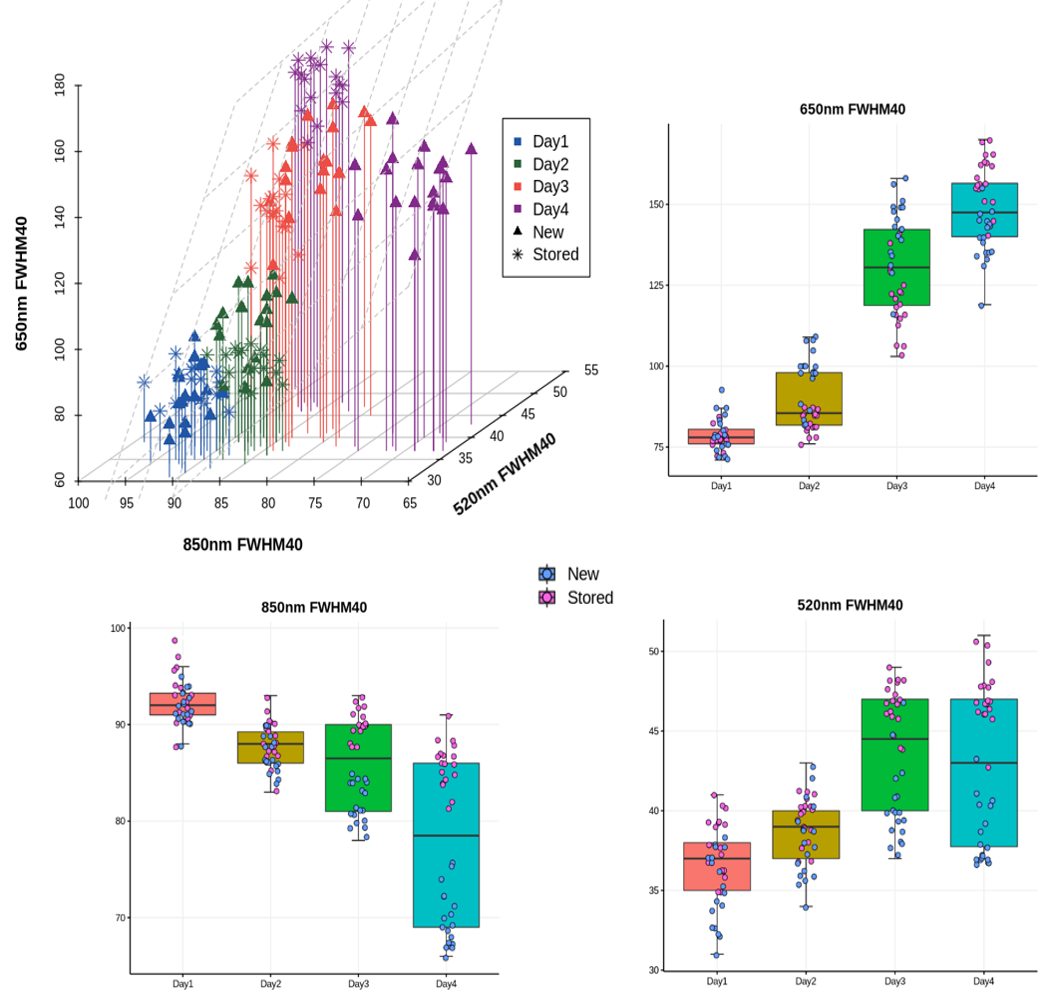
\includegraphics[width=13cm]{./Figure/SLB.png}
    \textbf{\caption{Spectral reflection signal of three channels when the broccoli heads naturally rot}\label{shelf}}{Spectral images were collected by a camera with 3 waveband filters (green, red and near-infrared) under stable LED illumination. By segmenting the background and using the median to represent the signal of the entire broccoli head. The spectral reflectance of the broccoli head changes significantly with its natural decay. Among the early spectral signals which we are more concerned, 520 nm and 850 nm bands seem to be more effective to distinguish the new and stored heads. However, in general, their non-linear variations in different signals are elusive, and further modeling is needed.}
\end{figure}
\noindent
Next, we placed the new and stored broccoli heads at room temperature, let them decay naturally to capture the shelf-life related signals. With time elapsing, the reflectivity of the three selected channels can somewhat reflect the rotting changes. However, our focus is more on the first two days before the broccoli heads showed obvious decay phenotype. Among the three selected channels (green, red and near-infrared), the newly harvested broccoli heads could not be effectively distinguished from the stored one. Further statistical modeling or deep learning strategies need to be explored


\section{DISCUSSION}
From the results of various VIs calculated in different treatments (Figure \ref{vif}), it seems not surprising that not getting a unified index that can effectively distinguish these four treatments, because of the complex relationship among them. However, detailed analysis can still give us some inspiration. Firstly, indices based on red and near-infrared such as RVI, NDVI and EVI, can somewhat reflect the physiological characteristics of plants, however, they are more used in the field of remote sensing for various kinds of local, regional, and global scale models, including general circulation and biogeochemical models \citep{peterson1988remote,huete2002overview}. While in CVI, CI-G, CI-RE these indices of leaf chlorophyll content \citep{gitelson2003relationships,vincini2008broad}, they seem to have a consistent result, except CI-RE, which doesn't consider the green channel. Results show that in the water-deficient environment (drought, heat\&drought), the chlorophyll content of broccoli leaves was significantly affected (CVI, CI-G). This water stress phenomenon has been extensively supported, and it's also well understood that lack of water hinders nutrient transport in plants and thus affects photosynthetic pigments synthesis. As for the water index (WI), it reflects water absorption in the mesophyll andd had been shown to have a good indication of water content in many crops \citep{wang2015determining,dawson1999propagation,penuelas1997estimation}. The result here is also very satisfactory, it can be seen that there were significant differences between the two treatments except drought and combined stress. This indicates that in heat stress, the water content of the plant leaves is also affected, even though they are well watered, and this effect is not sufficient to superimpose the significance in the combined stress relative to the drought stress.  The functional basis of the PRI is related on its sensitivity to rapid changes in carotenoids through the de-epoxidation of the xanthophyll pigments \citep{magney2016response}. It can serve as an indirect means for water stress detection due to the effects of water stress on the efficiency of photosynthesis. Researchers have demonstrated the sensitivity of PRI to short-term crop water stress detection \citep{gamon1997photochemical,suarez2010orchard,zarco2013pri}, and to the long-term change of carotenoid / chlorophyll ratio \citep{mand2010responses}. Here, we found that PRI is sensitive to the combination of drought and heat stress in broccoli, which may imply the cumulative effect of stress on photosynthetic efficiency and pigments. And of course, more studies is needed to support these inference.
\\
\\
In the process of machine learning model training for hyperspectral data, the results of feature engineering show that the important features are mainly concentrated in the green and near infrared (Figure \ref{dim},\ref{SL}).  In detail, because the hyperspectral bandwidth is small, there will inevitably be a lot of redundant information. Data dimensionality reduction can effectively extract important information, shorten model training time and reduce over-fitting. Here, dimensionality reduction by PCA can effectively de-correlate and remove the linear relationship between dimensions, but it does not consider the classification information. Therefore, after dimensionality reduction, the loss of information will be minimized, but classification may become more difficult (Figure \ref{dim}a). The data points in the graph are not clustering, and from the contribution of each component to the principal component (Figure \ref{dim}b), it's truly hard to get useful information. Another commonly used dimension reduction method is LDA, which seeks to distinguish data points as easily as possible after dimension reduction. After dimensionality reduction, the sample data has the largest inter-class distance and the smallest intra-class variance in the new dimension space, and the data has the best separability in the low dimension space (Figure \ref{dim}c). It can almost reach 100\% classification, so that the contribution of each wavelength may better explain the important features for classification, here are the green and red edges(Figure \ref{dim}d).
\\
\\
Then, as for feature selection, several methods of experimentation had a good consistency, that is, infrared waveband information might be relatively important for classification (Figure \ref{SL}). It may be suggested that changes in mesophyll cell structure, such as membrane structure, are more likely to affect spectrum reflection in leaves under heat and drought stress, while changes in pigments are less important to distinguish between them. In particular, through the dynamic visualization of the random feature search box, we can more clearly see the importance of features to the relationship between them (Figure \ref{SL}c). The water stress and control group showed the most significant difference around 700-900 nm, which was basically consistent with the WI. Wavelength around 700-800 nm may be important for distinguishing between heat stress and control. As for combined stress, it seems similar to the water stress. And between the combined stress and the individual stress, there is a difference around 420 nm.
\\
\\
Finally, the results of the four machine learning models show that linear classifier performs well when the data dimension is relatively large, while the tree model does not (Table \ref{auc}). This is understandable because regularization is used in training linear classifiers, which can effectively deal with multiple collinearity problems and reduce the weight of redundant information. The tree model can also be improved after dimensionality reduction. According to the statistical analysis results, we empirically select 409-429, 558-577, 700-896 and 926-967 nm waveband information for training, so we can see that the performance of the XGBoost model has been improved effectively, its AUC can reach 0.9096. By showing the confusion matrix (Figure \ref{CM}), it is not surprising that the control group and the combined stress group can achieve the best distinction. But surprisingly, the heat stress group can be more effectively distinguished from other stresses, as opposed to the drought group which may have more phenotype. The erroneous distinction of drought group mostly appears in the difference to control group, which may be explained to some extent that some of the leaves do not reach the threshold at which the drought can be detected.
\\
\\
As for the prediction of broccoli shelf life, due to the increasingly mature computer vision technology based on deep learning, and relatively stable environment and large data generated in production. It is easy to obtain high accuracy through a large number of data labeling and transfer learning. What is important is that for the capture of broccoli shelf life related signals, the more challenging is the signal difference in the early fresh period. Although we can get a signal that changes significantly with the decay of broccoli, how to predict its shelf life in the early stage remains to be further studied.
\section{Limitations and Future Research}
In the laboratory work, because planting broccolis requires a lot of time and space investment, limited by this, we have not been able to obtain large-scale image data and multibody repeated hyperspectral data. For the training of machine learning models and deep neural networks, they require a large amount of data, so more training data still needs to be acquired to train robust models.
\\
\\
The discussion of the specific molecular and physiological mechanisms for the results, most of them are extended through similar studies, and there could be differences between species and platforms. Further, for the pigment or physiological changes under complex stress of plants still need to be studied. To link the significant different spectral characteristics of complex stress with the changes of plant metabolites could be the direction of exploration.
\\
\\
Besides, for the relatively poor drought stress prediction effects. Error prediction is more likely to occur in control and combination stress (Figure \ref{CM}). The results could be due to the different degree of water stress on leaves. Collecting quantitative stress level data as dependent variable, turning classification problem into a regression problem could have better model performance.
\\
\\
While for predicting the shelf life of broccolis, it is feasible to make predictions from statistical signal differences, but as we see, predicting the shelf life of healthy broccoli heads with subtle difference requires more advanced technology and more data, and deep learning strategy is still the direction we need to develop.

\section{ACKNOWLEDGEMENTS}
\noindent
I'm very greatful to my supervisor Dr. Oliver Windram for his patient guidance on this project and meticulous feedback on the writing. I'm also greatful to Chris Adam for his guidance on how to use the spectrophotometer. Besides, many thanks for Sarah Blanford from Sainsbury's and James Brown from POLLYBELL FARMS LTD for their support on this project.

\section{CODE \& DATA ACCESSIBILITY}
All the code used for this project can be obtained from:\\
 \url{https://github.com/Luoxsh6/CMEECourseWork},\\
and the data from: \\
\url{https://imperialcollegelondon.box.com/s/k4ckuprv1if7kxqzb4lsiqhuxp22zwee}


\bibliography{Report}
    
\section{Supplementary Information}

\begin{figure}[H] 
    \centering 
    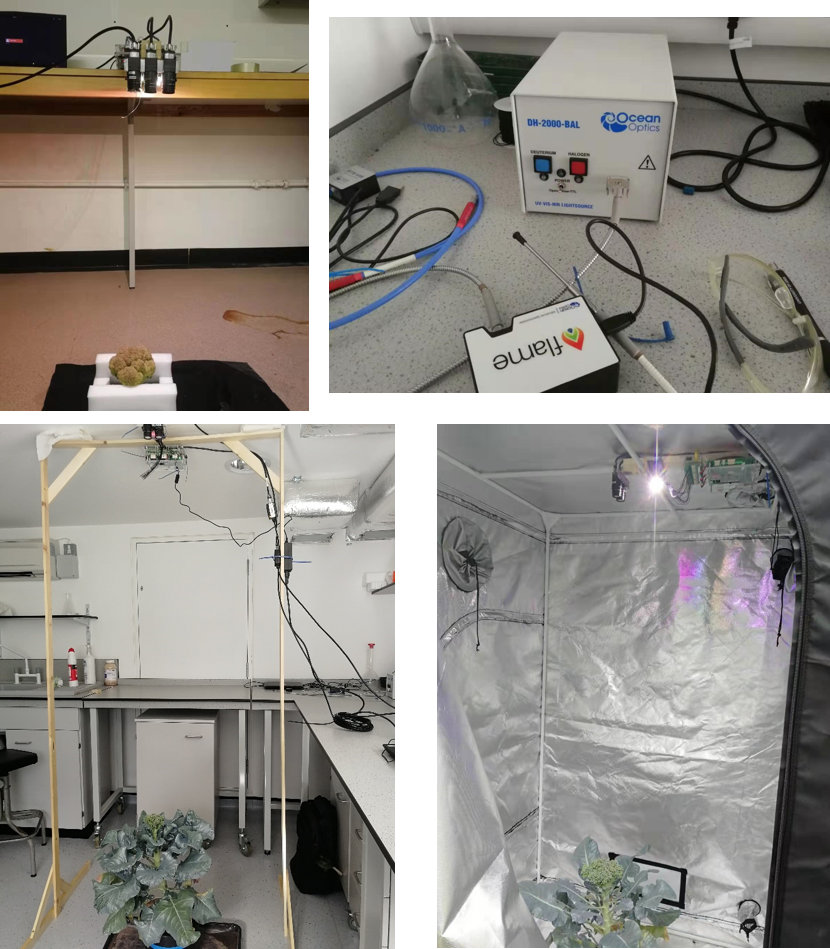
\includegraphics[width=8cm]{./Figure/SI1.png}
    \textbf{\caption{Experiment Apparatus}\label{si1}}{The tools used for images collection are basically consistent, spectral cameras with filters, spectrophotometer, LED lights and controllers. The figure shows the experiment apparatus for broccoli shelf life, broccoli in the control-environment room and in the grow tent.
    }
\end{figure}

\begin{figure}[H] 
    \centering 
    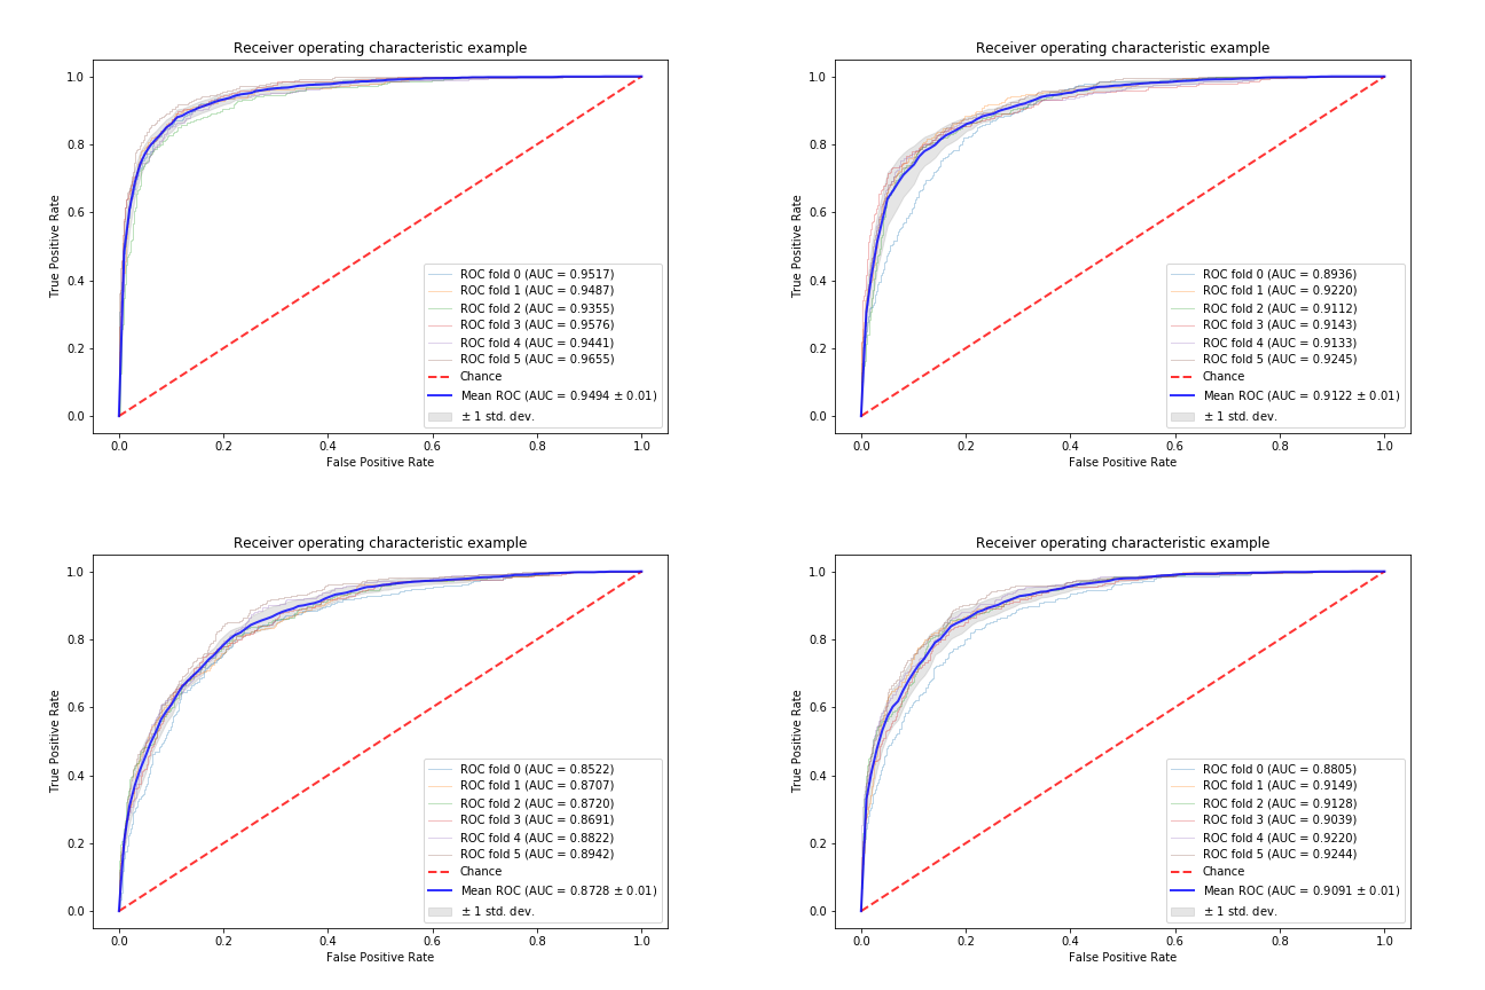
\includegraphics[width=13cm]{./Figure/SI3.png}
    \textbf{\caption{ROC for the best performance model}\label{si2}}{The ROC curve corresponding to the confusion matrix in the context}
\end{figure}

\begin{figure}[H] 
    \centering 
    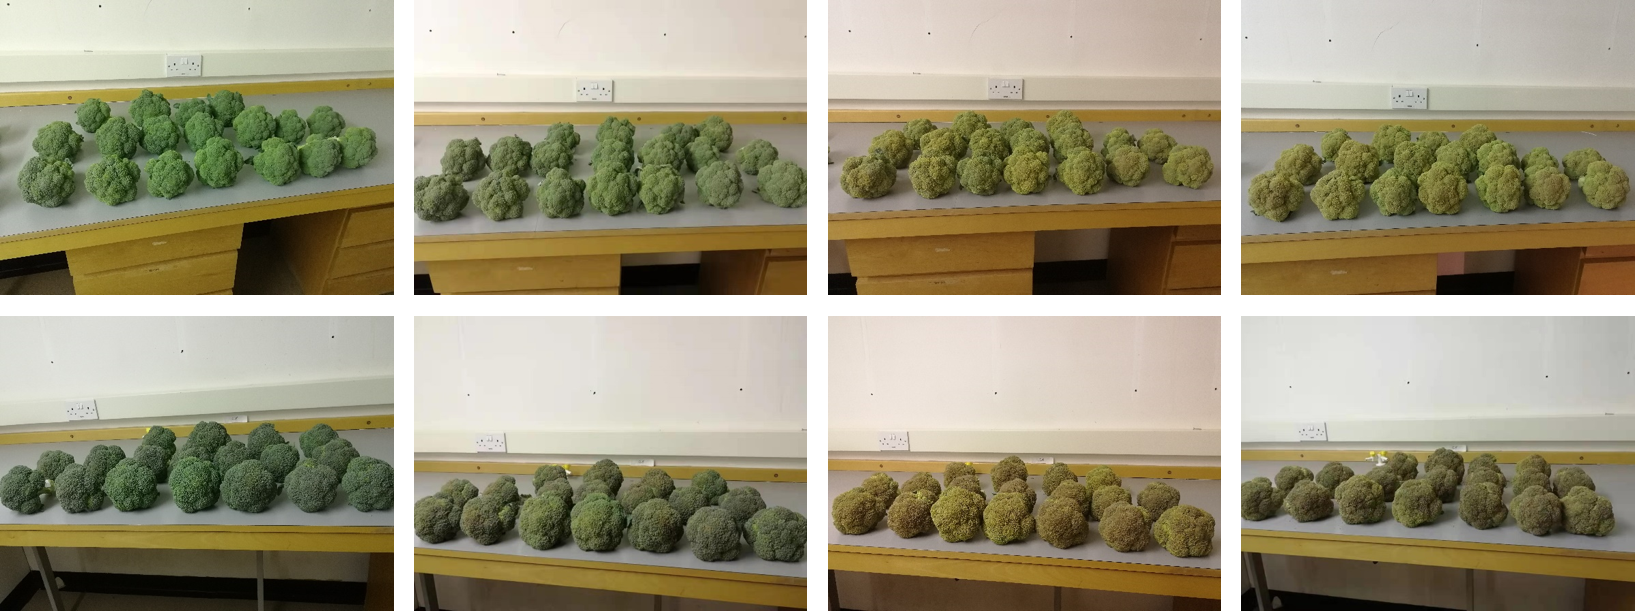
\includegraphics[width=13cm]{./Figure/SI2.png}
    \textbf{\caption{Broccoli status for shelf-live prediction}\label{si3}}{The RGB images of the naturally decaying broccoli, the images above is the broccoli stored for 2 weeks. The images below show the newly harvested broccoli, from left to right represent change of corresponding days.}
\end{figure}

\end{document}


        
    

